%%%%%%%%%%%%%%%%%%%%%%%%%%%%%%%%%%%%%%%%%%%%%%%%%%%%%%%%%%%%%%%%%%%%%%
% amspaper.tex --  LaTeX-based template for submissions to American 
% Meteorological Society journals
%
% Template developed by Amy Hendrickson, 2013, TeXnology Inc., 
% amyh@texnology.com, http://www.texnology.com
% following earlier work by Brian Papa, American Meteorological Society
%
% Email questions to latex@ametsoc.org.
%
%%%%%%%%%%%%%%%%%%%%%%%%%%%%%%%%%%%%%%%%%%%%%%%%%%%%%%%%%%%%%%%%%%%%%
% PREAMBLE
%%%%%%%%%%%%%%%%%%%%%%%%%%%%%%%%%%%%%%%%%%%%%%%%%%%%%%%%%%%%%%%%%%%%%

%% Start with one of the following:
% DOUBLE-SPACED VERSION FOR SUBMISSION TO THE AMS
\documentclass{ametsoc}

% TWO-COLUMN JOURNAL PAGE LAYOUT---FOR AUTHOR USE ONLY
% \documentclass[twocol]{ametsoc}

%%%%%%%%%%%%%%%%%%%%%%%%%%%%%%%%
%%% To be entered only if twocol option is used

\journal{jpo}

%  Please choose a journal abbreviation to use above from the following list:
% 
%   jamc     (Journal of Applied Meteorology and Climatology)
%   jtech     (Journal of Atmospheric and Oceanic Technology)
%   jhm      (Journal of Hydrometeorology)
%   jpo     (Journal of Physical Oceanography)
%   jas      (Journal of Atmospheric Sciences)	
%   jcli      (Journal of Climate)
%   mwr      (Monthly Weather Review)
%   wcas      (Weather, Climate, and Society)
%   waf       (Weather and Forecasting)
%   bams (Bulletin of the American Meteorological Society)
%   ei    (Earth Interactions)

%%%%%%%%%%%%%%%%%%%%%%%%%%%%%%%%
%Citations should be of the form ``author year''  not ``author, year''
\bibpunct{(}{)}{;}{a}{}{,}

%%%%%%%%%%%%%%%%%%%%%%%%%%%%%%%%

\usepackage{fancyref}

%%% To be entered by author:

%% May use \\ to break lines in title:

\title{Submesoscale streamers and the exchange water on the North Wall of the Gulf Stream}

%%% Enter authors' names, as you see in this example:
%%% Use \correspondingauthor{} and \thanks{Current Affiliation:...}
%%% immediately following the appropriate author.
%%%
%%% Note that the \correspondingauthor{} command is NECESSARY.
%%% The \thanks{} commands are OPTIONAL.

    \authors{Jody M. Klymak\correspondingauthor{Jody M.\ Klymak,
    School of Earth and Ocean Sciences ,
    University of Victoria,
    P.O. Box 3055 STN CSC
Victoria, BC Canada, V8W 3P6 }}
    \affiliation{University of Victoria, Victoria, Canada}
    
%    , R. Kipp Shearman$^2$, Craig M. Lee$^3$, Eric A. D'Asaro$^3$, Leif N. Thomas$^4$, Ramsey Harcourt$^3$, Andrey Scherbina$^3$, Miles A. Sundermeyer$^5$, Jeroen Molemaker$^6$, James C. McWilliams$^6$\& Johnathan Gula$^6$}
    
   
\email{jklymak@uvic.ca}


    \extraauthor{R. Kipp Shearman}
    \extraaffil{Oregon State University, Corvallis, Oregon, USA}
    \extraauthor{Craig M.\ Lee, Eric A. D'Asaro}
    \extraaffil{University of Washington, Seattle, Washington USA}
    \extraauthor{Leif N. Thomas}
    \extraaffil{Stanford University, Stanford, California, USA}
    \extraauthor{Ramsey Harcourt, Andrey Shcheribina}
    \extraaffil{University of Washington, Seattle, Washington USA}
    \extraauthor{Miles Sundermeyer}
    \extraaffil{University of Massachusetts, Bedford, Massachusetts, USA}
    \extraauthor{Jeroen Molemaker, James C. McWilliams, Johnathan Gula}
    \extraaffil{University of California, Los Angeles, California, USA }
    
    


%%%%%%%%%%%%%%%%%%%%%%%%%%%%%%%%%%%%%%%%%%%%%%%%%%%%%%%%%%%%%%%%%%%%%
% ABSTRACT
%
% Enter your Abstract here

\abstract{The Gulf Stream is a major conduit of warm surface water from the tropics to the subpolar Atlantic.  It retains its unique temperature and salinity properties for hundreds of kilometers, as the strongly sheared "North Wall" acts as a dynamical barrier to lateral mixing \cite{marshalletal06}.  Large mesoscale ($>20$ km) "rings" often pinch off, but like the Gulf Stream they are resistant to lateral mixing, and retain their properties for a long time.  Here we demonstrate one sub-mesoscale ($<20$ km) mechanism by which the Gulf Stream exchanges water with the cold subpolar water to the north, a series of "streamers" that detrain partially mixed water from the Gulf Stream at the top of meanders. These streamers entrain cold fresh water into the Gulf Stream, an important step in closing the salinity budget for the Stream noted by previous work \cite{joyceetal13}.
} 

\begin{document}


%% Necessary!
\maketitle


%%%%%%%%%%%%%%%%%%%%%%%%%%%%%%%%%%%%%%%%%%%%%%%%%%%%%%%%%%%%%%%%%%%%%
% MAIN BODY OF PAPER
%%%%%%%%%%%%%%%%%%%%%%%%%%%%%%%%%%%%%%%%%%%%%%%%%%%%%%%%%%%%%%%%%%%%%
%
\section{Introduction}
The Gulf Stream is the western boundary current of the North Atlantic wind-driven circulation.  It separates from Cape Hatteras and extends into the interior North Atlantic traveling east.  As it does so, it loses heat to the north, warming the subpolar gyre.  It also entrains water from both the north and south, increasing its eastward transport by approximately XX Sv/100 km.  It cools, primarily from atmospheric forcing due to evaporation and sensible heat exchange \cite{joyceetal13}.  

Despite being heavily studied, there are a number of things poorly understood about the Gulf Stream.  First, there is a very sharp temperature-salinity front on the northern wall.  Salinity decreases by almost 1.5 psu moving north across the front, compensated by a drop in temperature of almost $5\mathrm{^oC}$.   The sharpness of this front persists for 100s of kilometers, which is remarkably persistent.  The front happens along constant density surfaces which usually are not a barrier to mixing, however, the Gulf Stream water has very high potential vorticity (angular momentum), and thus does not tend to mix with the low potential vorticity water, at least on large scales \citep{marshalletal06}.  

Regardless of this vorticity barrier and the presence of the sharp stable front, budgets of properties of the Gulf Stream indicate that there must be significant exchange across the North Wall. \citet{joyceetal13} find that there must be a flux of X Sv of fresh water across the Gulf Stream.  This fresh water is necessary to create the dynamically important "18 degree water" that fills much of the upper Sargasso Sea.  This water is also cold and contributes to the cooling of the Gulf Stream, but it is not as important as the atmospheric forcing.  

Here we demonstrate that there is indeed small scale mixing at the base of the Gulf Stream, and that this water periodically peels off the Gulf Stream in thin sub mesoscale ``streamers''.  The streamers carry partially mixed warm, salty, and high vorticity  water north of the stream.  Because they have a cyclonic vorticity anomaly, they also wrap up cold fresh water and entrain it into the Stream.  The preferential detrainment of partially mixed water explains the persistent sharpness of the Gulf Stream front despite the presence of mixing processes at the base of the Stream.  We also speculate that the preferential detrainment of this water into the streamers is dynamically linked to the partial mixing of vorticity at the base of the Gulf Stream. The entrainment of cold fresh water is quantified to be approximately the right amount to close the salinity budget posed by \citet{joyceetal13}.  

\section{Setting}

In Mar 2012 we made detailed measurements of the North Wall of the Gulf Stream from 66 W to 60 W (\fref{fig:SatOverviewSectD}), about 850 km east of where the stream separates from the North American continental slope.  Two research vessels followed a Lagrangian float placed in the Gulf Stream front at $\sigma_{\theta}=XX\ \mathrm{kg\,m^{-3}}$.  The float was advected downstream with an average (and relatively constant) speed of 1.4 $\mathrm{m\,s^{-1}}$. It progressively moved to denser water as the Stream cooled downstream.  One vessel maintained a tight sampling of the float and deployed an undulating profiler to 200 m, making 10-km wide cross sections every 10 km downstream.  The second vessel also had an undulating profiler operating on a larger 30-km scale in the cross and along stream directions.  Both profilers measured temperature, salinity and pressure, and had approximately 1-km lateral resolution; both ships also measured ocean currents.  By following the float a unique focus on the front could be maintained as the front curved and meandered to the east.  


For the deployment discussed here, a shallow convex meander was followed (65 W, \fref{fig:SatOverviewSectD}b), followed by a long shallow concave region (63 W) before the float passed over a large convex meander (61 W).  Satellite measurements of sea surface temperature show the sharp temperature changes across the front, but they also show thin intermediate-temperature streamers detraining to the north at approximately 65 W, 64 W, and at the top of the large meander at 61 W.  A feature we expect was older can also be seen at 62 W with a clear rolled up signature.  The ships passed through the three newer streamers giving the first observation of these streamer's underwater structure.  

The shipboard data captures the structure of the Gulf Stream front and the streamers beneath the sea surface (\fref{fig:ThreeDSectionDAnnotate}).  Constant density surfaces slope up towards the north (\fref{fig:ThreeDSectionDAnnotate}b; contours in upper cross sections).  Salinity (coloured) along the density surfaces is very salty (and warm) in the Gulf Stream, and fresher and colder to the north.  The lateral contrast between the two waters is amongst the sharpest in the ocean, with salinity changing almost 1 psu over 5 km.  The temperature-salinity relationship has two dominant ``populations'' (\fref{fig:ThreeDSectionDAnnotate}c), with most of the observations falling on the ``North'' side of the GS or in the GS.  There is a small distinct population between that we term the ``Streamers''.  These manifest themselves in the cross-sections as intermediate salinity anomalies ($S \approx 36.15\ \mathrm{psu}$; \fref{fig:ThreeDSectionDAnnotate}b).   Along $\sigma_{\theta}=26.25\ \mathrm{kg\,m^{-3}}$, these anomalies are horizontally connected, and stream off the north wall of the Gulf Stream, and are stretched out for almost 50 km along the wall and are  about 10 km wide.  


Four example cross sections and an interpolation of the streamer temperature along the $\sigma_{\theta}=26.25\ \mathrm{kg\,m^{-3}}$ potential density surface show that a streamer that separates at approximately $64 W$. (\fref{fig:ThreeDSectionDAnnotate}b)


originate as water that is deeper than 100 m and directly under the sharp T/S front (\fref{fig:ThreeDSectionDAnnotate}b).  Looking upstream, the streamers detach from the base of the Gulf Stream and are advected north, and rise along isopycnals to the surface.  The structure at depth is more sharply delineated than the surface structure, which has been modified by atmospheric forcing; distinctive interleaving of high and low salinities is clearly seen between $\sigma_{\theta}=26.25\ \mathrm{kg\,m^{-3}}$ and $\sigma_{\theta}=26.5\ \mathrm{kg\,m^{-3}}$.  The streamers are order 5 km thick, and are made up of water intermediate to the water in the Gulf Stream and to the north, as clearly seen in T/S space (\fref{fig:SatOverviewSectD}c).  Water intermediate to two water masses is indicative of mixing, so there is mixing between the Gulf Stream water and water to the north, the nature of which is under study (references).






% TODO: Need to do a good job of showing the entrainment of cold water.

% TODO: Need to better quantify water flux out of GS.  i.e. do precisely with TS class and velocities.  



\begin{figure*}[htbp]
  \centering
    \includegraphics[width=\textwidth]{./SatOverviewSecD.pdf}
   \caption{{\bf Experimental design.}  a) The experiment site on the north wall of the Gulf Stream, between 66 and 60 W, as shown in this AVHRR satellite image of sea surface temperature (SST) (CITE??).  b) Detailed SST image composited from two satellites.  The Gulf Stream is warm and delineated by a sharp front.  There are small sub-mesoscale structures north of the front, which are the focus of this paper.  The front was sampled with two ships (\emph{R/V Knorr} and \emph{R/V Atlantis}) following a Lagrangian float \cite{dasarolien00a,dasaroetal11} which moved downstream in the front at an average speed of $1.4\ \mathrm{m\,s^{-1}}$. The ships each had undulating conductivity, temperature, and depth probes (CTDs), with the \emph{R/V Knorr} tracking the float within 10 km of the front, and the \emph{R/V Atlantis} providing larger-scale surveys of approximately 30 km cross-front distance.  Each profiler collected a depth profile to 200 m approximately every 1 km in the horizontal.  The float was emplaced at 17:07 5 Mar 2012, and followed for four days along the front. The satellite images are a composite from early in that period (AVHRR 6 Mar), and late in that period (MODIS, 9 Mar) c) The winds were strong ($>20\ \mathrm{m\,s^{-1}}$), from the northwest for the first two days, before swinging around to coming from the SE.  The strong winds and cool temperatures led to a net negative heat flux for most of the observation period. \label{fig:SatOverviewSectD} }
\end{figure*}

\begin{figure*}[htbp]
  \centering
    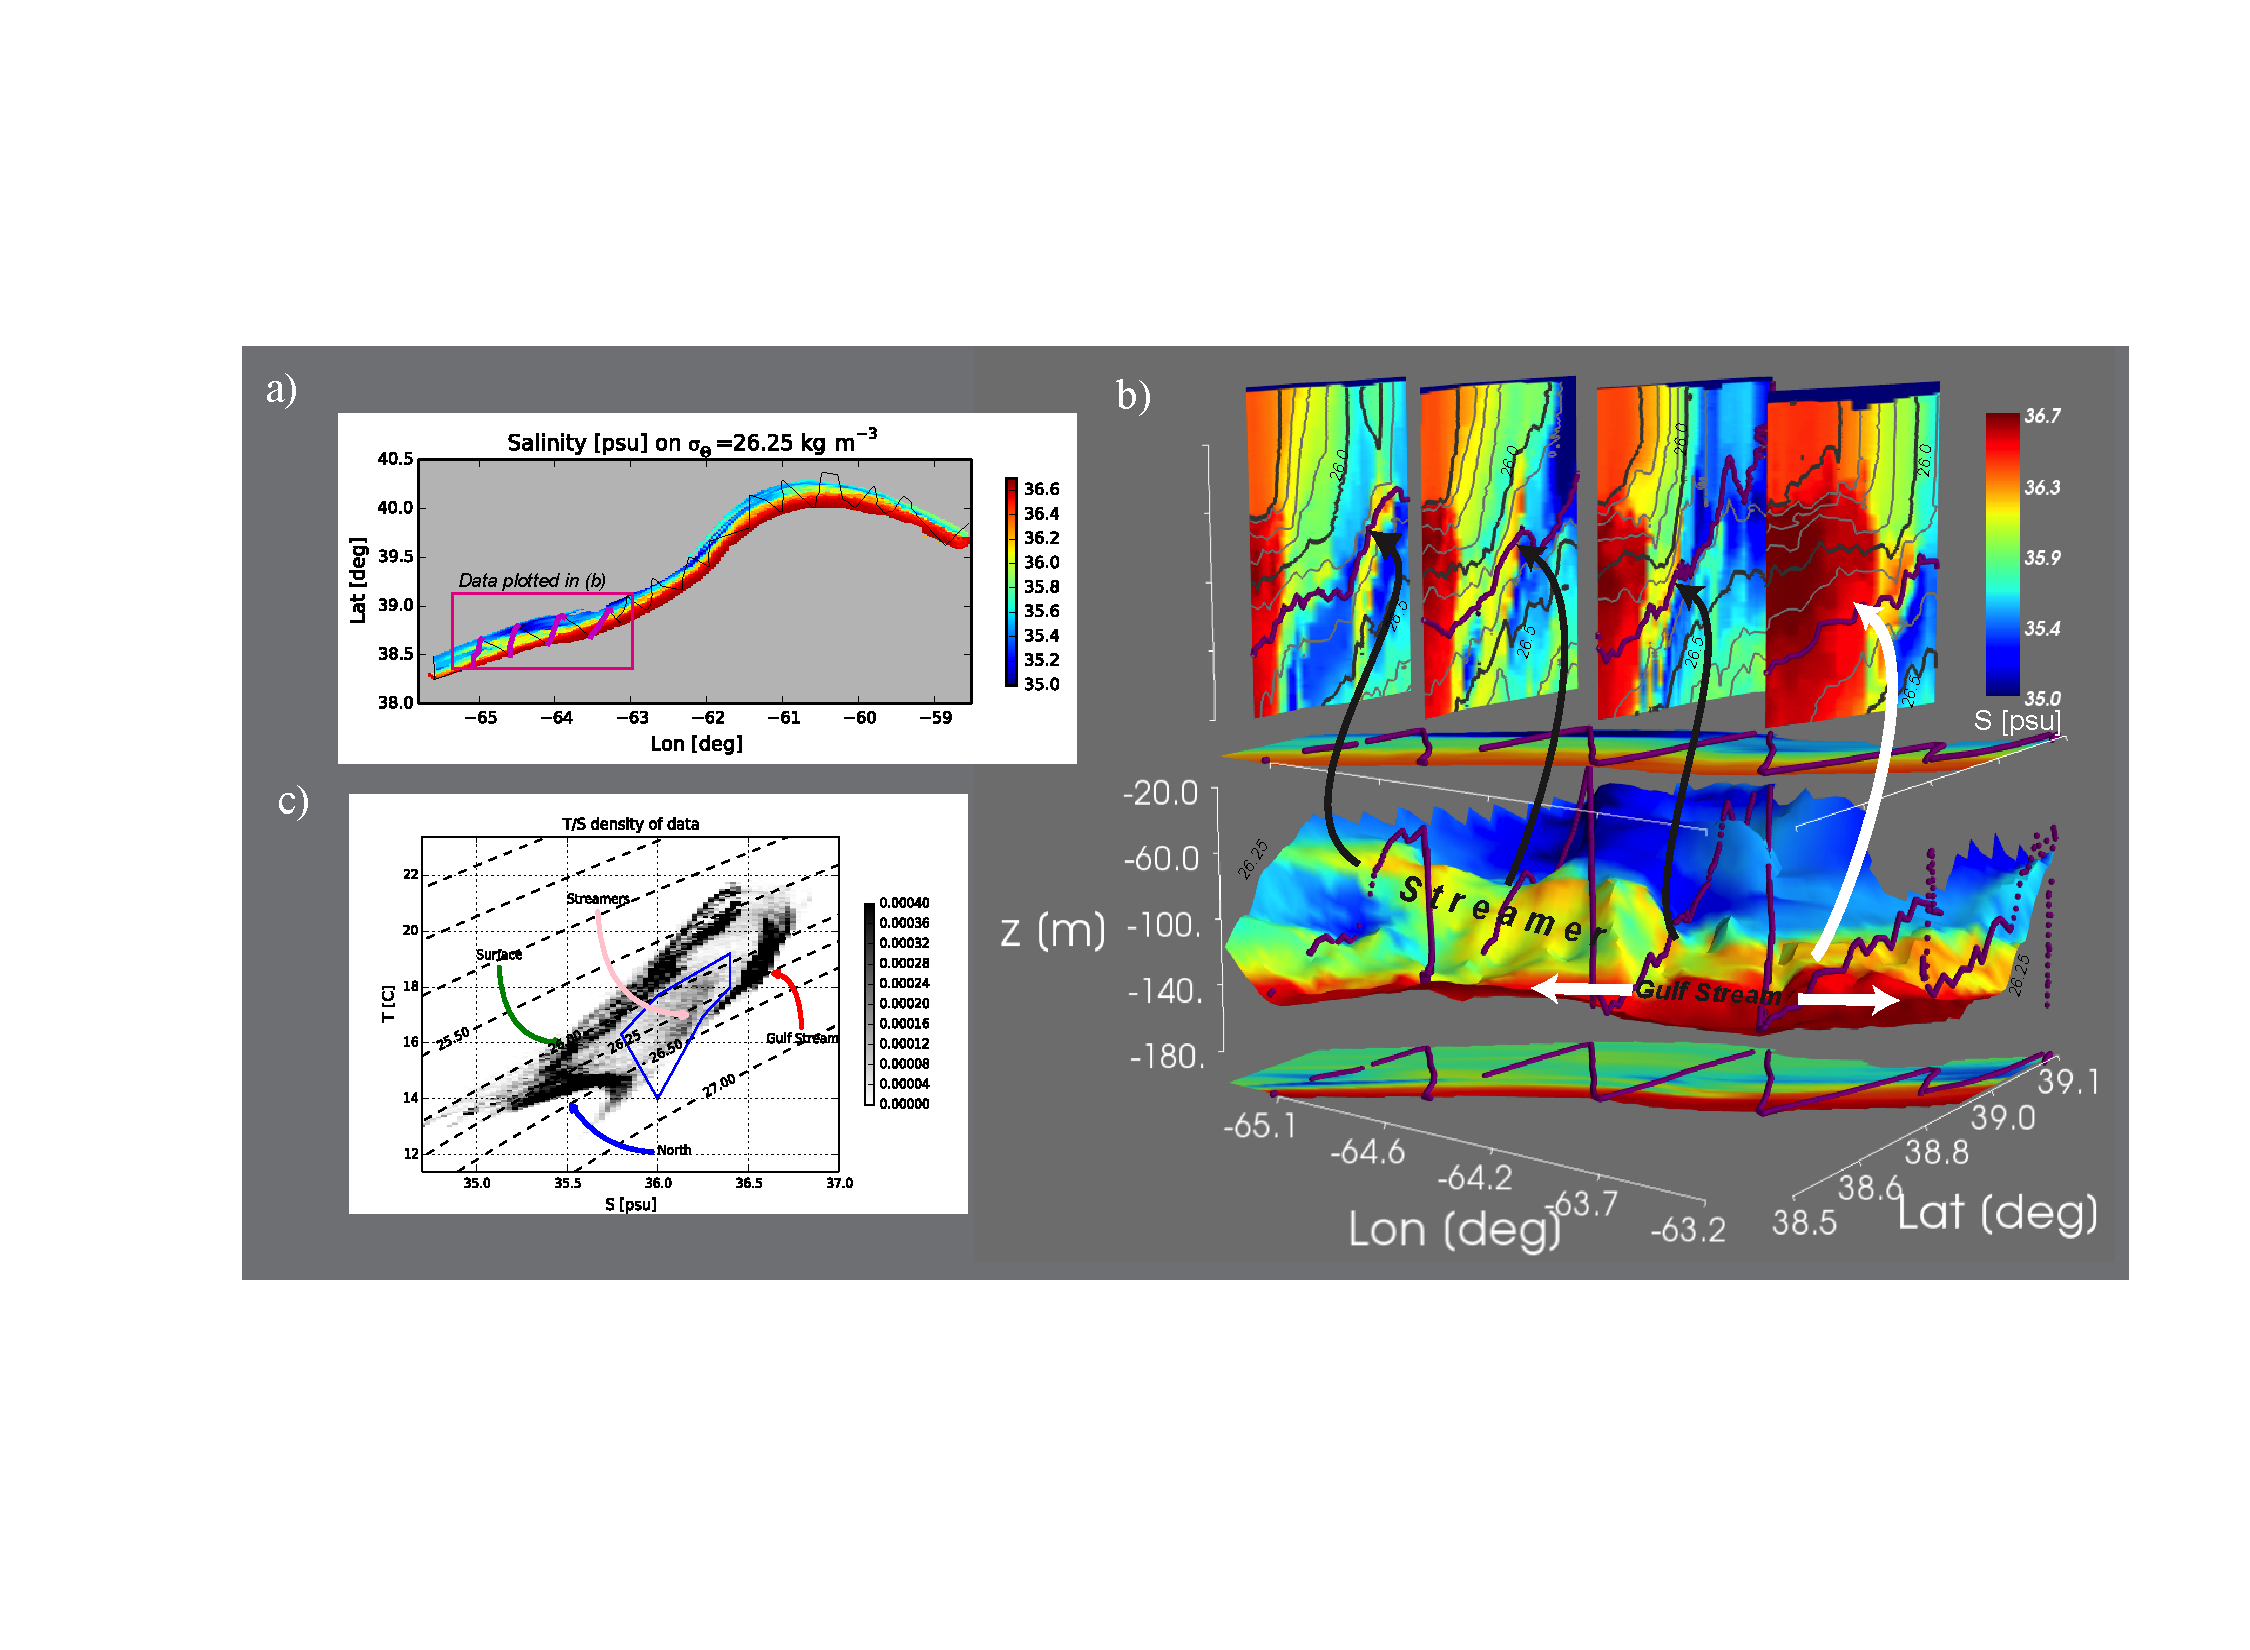
\includegraphics[width=\textwidth]{./ThreeDSectionDAnnotate.pdf}
   \caption{{\bf Streamers on the North Wall of the Gulf Stream.}  The upper sections salinity coloured on depth/cross-stream surfaces.  Black contours are constant-density surfaces. The dark-purple contour is \st{24.25}, and is the surface shown as a shaded projection in the lower representation of the same data.  Here salinity has been coloured at the depth of this constant-density surface.  The ship path is indicated on this surfaces, and the flat surface above and below.  
         }\label{fig:ThreeDSectionDAnnotate} 
 
\end{figure*}



\bibliographystyle{ametsoc2014}
\bibliography{main}
 
 
\end{document}
%
%%%%%%%%%%%%%%%%%%%%%%%%%%%%%%%%%%%%%%%%%%%%%%%%%%%%%%%%%%%%%%%%%%%%%%
%% TABLES
%%%%%%%%%%%%%%%%%%%%%%%%%%%%%%%%%%%%%%%%%%%%%%%%%%%%%%%%%%%%%%%%%%%%%%
%\begin{table}[h]
%\caption{This is a sample table caption and table layout.}\label{t1}
%\begin{center}
%\begin{tabular}{ccccrrcrc}
%\topline
%$N$ & $X$ & $Y$ & $Z$\\
%\midline
% 0000 & 0000 & 0010 & 0000 \\
% 0005 & 0004 & 0012 & 0000 \\
% 0010 & 0009 & 0020 & 0000 \\
% 0015 & 0016 & 0036 & 0002 \\
% 0020 & 0030 & 0066 & 0007 \\
% 0025 & 0054 & 0115 & 0024 \\
%\botline
%\end{tabular}
%\end{center}
%\end{table}
%%
%
%\begin{table}
%\appendcaption{A1}{Here is the appendix table caption.}
%\centering
%\begin{tabular}{ccc}
%\topline
%$1$ & $2$ & $3$ \\
%\midline
%a&b&c \\
%d&e&f \\
%\botline
%\end{tabular}
%\end{table}
%
%%%%%%%%%%%%%%%%%%%%%%%%%%%%%%%%%%%%%%%%%%%%%%%%%%%%%%%%%%%%%%%%%%%%%%
%% FIGURES
%%%%%%%%%%%%%%%%%%%%%%%%%%%%%%%%%%%%%%%%%%%%%%%%%%%%%%%%%%%%%%%%%%%%%%
%\begin{figure}[h]
% \centerline{\includegraphics[width=19pc]{figure01.pdf}}
%  \caption{Enter the caption for your figure here.  Repeat as
%  necessary for each of your figures. Figure from \protect\cite{Knutti2008}.}\label{f1}
%\end{figure}
%
%\begin{figure}
%\centerline{(illustration here)}
%\appendcaption{A1}{Here is the appendix figure caption.}
%\end{figure}
%
%\begin{figure}
%\centerline{(illustration here)}
%\appendcaption{B1}{Here is the appendix figure caption.}
%\end{figure}
%



%%%%%%%%%%%%%%%%%%%%%%%%%%%%%%%%%%%%%%%%%%%%%%%%%%%%%%%%%%%%%%%%%%%%%
% END OF AMSPAPER.TEX
%%%%%%%%%%%%%%%%%%%%%%%%%%%%%%%%%%%%%%%%%%%%%%%%%%%%%%%%%%%%%%%%%%%%%